
%(BEGIN_QUESTION)
% Copyright 2007, Tony R. Kuphaldt, released under the Creative Commons Attribution License (v 1.0)
% This means you may do almost anything with this work of mine, so long as you give me proper credit

Identify the control strategy represented in each of these block diagrams:

$$\includegraphics[width=15.5cm]{i01773x01.eps}$$

$$\includegraphics[width=15.5cm]{i01773x02.eps}$$

$$\includegraphics[width=15.5cm]{i01773x03.eps}$$

$$\includegraphics[width=15.5cm]{i01773x04.eps}$$


\underbar{file i01773}
%(END_QUESTION)





%(BEGIN_ANSWER)

In order from first to last:

\begin{itemize}
\item{} Cascade 
\item{} (Pure) feedforward
\item{} Feedforward with trim
\item{} Ratio
\end{itemize}

%(END_ANSWER)





%(BEGIN_NOTES)

In the first system, there is a feedback control loop inside of another feedback control loop.  This is cascade.
 
\vskip 10pt

In the second system, there is no feedback of the controlled variable at all.  Rather, the load ($q$) is sensed and action taken on that measurement.  This is feedforward control in its simplest (and least practical) form.
 
\vskip 10pt

In the third system, a two cascaded control loops receive feedforward action from a measurement taken on the load of process \#2 ($q_2$).  This is feedforward+feedback control, also known as three-element control (note the three measurements acted upon in this system: $C_1$, $C_2$, and $q_2$).
 
\vskip 10pt

In the fourth system, an uncontrolled variable from one process ($u$) establishes a setpoint for the controlled variable of another process.  The multiplier block ($\times$) establishes the ratio between the two variables.

%INDEX% Documentation, block diagram: control strategy

%(END_NOTES)


